\documentclass{beamer}
\usepackage{amsmath}
\usepackage{graphicx}
\usepackage{listings}
\usepackage{subfig}
\usepackage{hyperref}
\usepackage{tcolorbox,fancyvrb,xcolor,tikz}
\tcbuselibrary{skins,breakable}

\newenvironment{VerbatimIN}
 {\VerbatimEnvironment
  \begin{tcolorbox}[
    breakable,
    colback=lightgray,
    spartan
  ]%
  \begin{Verbatim}}
 {\end{Verbatim}\end{tcolorbox}}

 \newenvironment{VerbatimOUT}
 {\VerbatimEnvironment
  \begin{tcolorbox}[
    breakable,
    spartan
  ]%
  \begin{Verbatim}}
 {\end{Verbatim}\end{tcolorbox}}


\title{Mixed Effects Models - Week 6}
\subtitle{Praxis and Fitting of Mixed Effects Models in R}
\author{Marieke Wesselkamp\\Department of Biometry and Environmental Systems Analysis\\Albert-Ludwigs-University of Freiburg (Germany)}
\date{November 2024}

\begin{document}

\frame{\titlepage}

\begin{frame}
    \frametitle{The Linear Mixed Effects Model}
    \[
    \mathbf{y} = \mathbf{X} \cdot \mathbf{b} + \mathbf{Z} \cdot \mathbf{u} + \mathbf{e}
    \]
    \[
    \mathbf{e} \sim \mathcal{N}(0, \mathbf{R}), \quad \mathbf{u} \sim \mathcal{N}(0, \mathbf{G}), \quad \mathbf{u} \bot \mathbf{e}
    \]
    where:
    \begin{itemize}
        \item $\mathbf{y}$: measured response values
        \item $\mathbf{X}$: Fixed Effects design matrix
        \item $\mathbf{b}$: Fixed Effects parameter vector of $\mathbf{X}$
        \item $\mathbf{e}$: Vector of the errors $\epsilon$, which are normally distributed (mean = 0; variance by residual variance-covariance matrix \textbf{R})
    \end{itemize}
\end{frame}

\begin{frame}
    \frametitle{Stochastic Components of Mixed Effects Models}
    \begin{itemize}
        \item The \textbf{first stochastic part} describes how random effects parameters $\mathbf{u}$ vary around 0 and is given by the random effects variance-covariance matrix \textbf{G}
        \[
        \mathbf{u} \sim \mathcal{N}(0, \mathbf{G})
        \]
        \item The \textbf{second stochastic part} describes the remaining and unexplained (\textit{residual}) variance:
        \[
        \mathbf{e} \sim \mathcal{N}(0, \mathbf{R})
        \]
        It describes how the measurements \textbf{e} vary around 0, \textbf{After} accounting for the fixed and random effects and is given by the residual variance-covariance matrix \textbf{R}.
    \end{itemize}
\end{frame}
\begin{frame}[fragile]
    \textbf{The size (distance) of 16 boys and 11 girls measured 4 times at ages 8, 10, 12, 14}
    \scriptsize
    \begin{VerbatimIN}[numbers=left,numbersep=6pt]
str(Orthodont, give.attr = FALSE, vec.length = 2)        
    \end{VerbatimIN}[numbers=left,numbersep=6pt]
    \tiny
    \begin{VerbatimOUT}[numbers=left,numbersep=6pt]
Classes 'nfnGroupedData', 'nfGroupedData', 'groupedData' and 'data.frame':
 108 obs. of  4 variables:
 $ distance: num  26 25 29 31 21.5 22.5 23 26.5 23 22.5 ...
 $ age     : num  8 10 12 14 8 10 12 14 8 10 ...
 $ Subject : Ord.factor w/ 27 levels "M16"<"M05"<"M02"<..: 15 15 15 15 3 3 3 3 7 7 ...
 $ Sex     : Factor w/ 2 levels "Male","Female": 1 1 1 1 1 1 1 1 1 1 ...
    \end{VerbatimOUT}[numbers=left,numbersep=6pt]

    \normalsize\textbf{Subject and Sex as categorical, distance and age as continous variables}
    \scriptsize
    \begin{VerbatimIN}[numbers=left,numbersep=6pt]
xtabs(~Sex+age, Orthodont)
    \end{VerbatimIN}[numbers=left,numbersep=6pt]
    \begin{VerbatimOUT}[numbers=left,numbersep=6pt]
        age
Sex       8 10 12 14
  Male   16 16 16 16
  Female 11 11 11 11
    \end{VerbatimOUT}[numbers=left,numbersep=6pt]
    \normalsize\textbf{Unbalanced, full-factorial, always same age values}
\end{frame}

\begin{frame}[fragile]
    \frametitle{Data Plot: Distance vs Age}
    \textbf{The size (distance) of 16 boys and 11 girls measured 4 times at ages 8, 10, 12, 14}
    \scriptsize
    \begin{VerbatimIN}[numbers=left,numbersep=6pt]
xyplot(distance ~ age|Sex, groups = Subject, type = "o")        
    \end{VerbatimIN}[numbers=left,numbersep=6pt]
    \begin{center}
    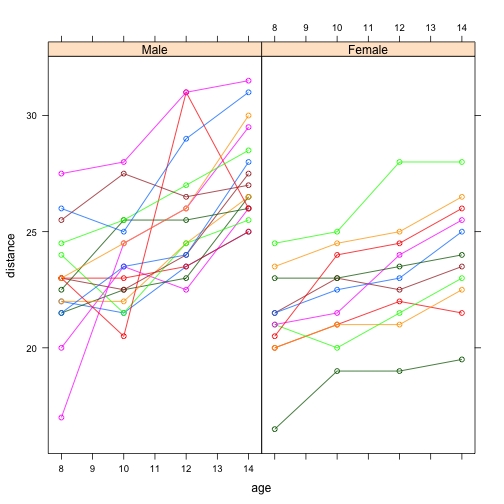
\includegraphics[width=0.55\textwidth]{lectures/day_6_praxis_and_fitting_of_mems/figures/unnamed-chunk-3-1.png} 
    \end{center}
\end{frame}


\begin{frame}[fragile]
    \frametitle{Avoidance of LMM I: Taking Averages}
    \begin{columns}
        \begin{column}{0.65\textwidth}
        \scriptsize
        \begin{VerbatimIN}[numbers=left,numbersep=6pt]
dist <- tapply(distance, Subject, mean)
sex <- as.factor(c(rep("boy", 16), 
                   rep("girl", 11)))
mod <- lm(dist ~ sex)
summary(mod)$coef            
        \end{VerbatimIN}[numbers=left,numbersep=6pt]
        \tiny
        \begin{VerbatimOUT}[numbers=left,numbersep=6pt]
             Estimate Std. Error   t value     Pr(>|t|)
(Intercept) 24.968750  0.4860008 51.375949 7.154854e-27
sexgirl     -2.321023  0.7614168 -3.048294 5.375056e-03
        \end{VerbatimOUT}[numbers=left,numbersep=6pt]
        \end{column}
        \begin{column}{0.35\textwidth}
            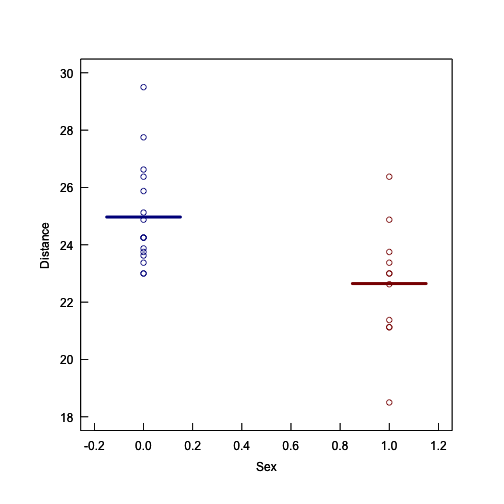
\includegraphics[width=\textwidth]{lectures/day_6_praxis_and_fitting_of_mems/figures/unnamed-chunk-5-1.png}
        \end{column}
    \end{columns}
    \vspace{0.5cm}
    
    \textbf{Loss of information: no age-effect anymore!}
\end{frame}

\begin{frame}[fragile]
    \frametitle{Avoidance of LMM II: Ignoring grouping}
    \textit{aka complete pooling}
    \begin{columns}
        \begin{column}{0.65\textwidth}
        \scriptsize
        \begin{VerbatimIN}[numbers=left,numbersep=6pt]
mod <- lm(dist ~ I(age-8) * Sex)
summary(mod)$coef[,c(1:2,4)]            
        \end{VerbatimIN}[numbers=left,numbersep=6pt]
        \tiny
        \begin{VerbatimOUT}[numbers=left,numbersep=6pt]
                       Estimate Std. Error     Pr(>|t|)
(Intercept)          22.6156250  0.4720747 1.060063e-72
I(age - 8)            0.7843750  0.1261673 1.069216e-08
SexFemale            -1.4065341  0.7395990 5.997069e-02
I(age - 8):SexFemale -0.3048295  0.1976661 1.260761e-01    
        \end{VerbatimOUT}[numbers=left,numbersep=6pt]
        \scriptsize
        \begin{VerbatimIN}[numbers=left,numbersep=6pt]
summary(mod)$df[1:2]            
        \end{VerbatimIN}[numbers=left,numbersep=6pt]
        \begin{VerbatimOUT}[numbers=left,numbersep=6pt]
[1]   4 104            
        \end{VerbatimOUT}[numbers=left,numbersep=6pt]
        \end{column}
        \begin{column}{0.35\textwidth}
            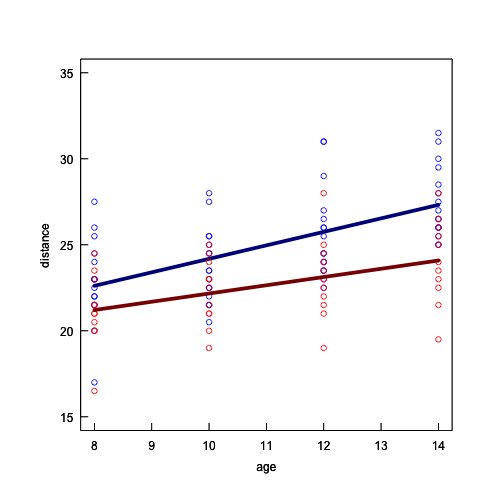
\includegraphics[width=\textwidth]{lectures/day_6_praxis_and_fitting_of_mems/figures/unnamed-chunk-7-1.png}
        \end{column}
    \end{columns}
\end{frame}

\begin{frame}[fragile]
    \frametitle{Avoidance of LMM III: Covariate}
    \textit{Child as covariate (= no pooling)}
    \begin{columns}
        \begin{column}{0.65\textwidth}
        \scriptsize
        \begin{VerbatimIN}[numbers=left,numbersep=6pt]
mod <- lm(distance ~ I(age-8)*Sex*Subject)
head(summary(mod)$coef)[,c(1:2,4)]
        \end{VerbatimIN}[numbers=left,numbersep=6pt]
        \tiny
        \begin{VerbatimOUT}[numbers=left,numbersep=6pt]
                Estimate Std. Error     Pr(>|t|)
(Intercept)  30.46129230  2.6433633 3.568372e-16
I(age - 8)   -0.00244428  0.7064685 9.972522e-01
SexFemale   -20.66408111  6.4675643 2.335693e-03
Subject.L    46.02266626 14.1052771 1.915757e-03
Subject.Q     9.78302300  3.5449564 7.883933e-03
Subject.C   -11.26155483  4.5924662 1.746278e-02
        \end{VerbatimOUT}[numbers=left,numbersep=6pt]
        \scriptsize
        \begin{VerbatimIN}[numbers=left,numbersep=6pt]
summary(mod)$df[1:2]            
        \end{VerbatimIN}[numbers=left,numbersep=6pt]
        \begin{VerbatimOUT}[numbers=left,numbersep=6pt]
[1] 54 54            
        \end{VerbatimOUT}[numbers=left,numbersep=6pt]
        \end{column}
        \begin{column}{0.35\textwidth}
            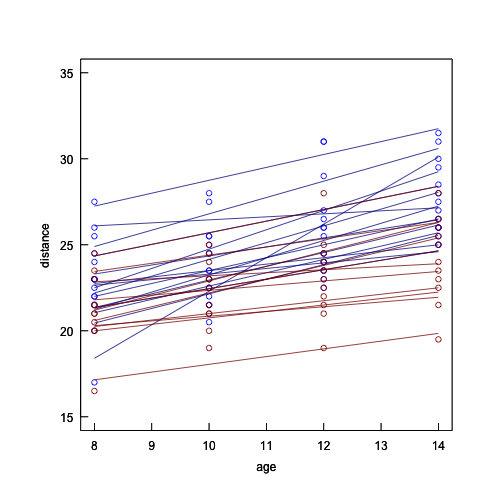
\includegraphics[width=\textwidth]{lectures/day_6_praxis_and_fitting_of_mems/figures/unnamed-chunk-9-1.png}
        \end{column}
    \end{columns}
    \vspace{0.5cm}
\end{frame}

\begin{frame}[fragile]
    \frametitle{Avoidance of LMM IV: fitting a "marginal" gls model}
    \tiny
    \begin{VerbatimIN}[numbers=left,numbersep=6pt]
mod.gls <- gls(distance ~ I(age-8) * Sex, 
               correlation = corAR1(form = ~ 1|Subject))
summary(mod.gls)        
    \end{VerbatimIN}[numbers=left,numbersep=6pt]
    \begin{VerbatimOUT}[numbers=left,numbersep=6pt]
Generalized least squares fit by REML
  Model: distance ~ I(age - 8) * Sex 
  Data: NULL 
       AIC      BIC    logLik
  456.5874 472.4538 -222.2937
Correlation Structure: AR(1)
 Formula: ~1 | Subject 
 Parameter estimate(s):
      Phi 
0.6244888 
Coefficients:
                         Value Std.Error  t-value p-value
(Intercept)          22.753181 0.5617321 40.50540  0.0000
I(age - 8)            0.769263 0.1169509  6.57766  0.0000
SexFemale            -1.562071 0.8800650 -1.77495  0.0788
I(age - 8):SexFemale -0.285443 0.1832268 -1.55787  0.1223
 Correlation: 
                     (Intr) I(g-8) SexFml
I(age - 8)           -0.625              
SexFemale            -0.638  0.399       
I(age - 8):SexFemale  0.399 -0.638 -0.625
Standardized residuals:
        Min          Q1         Med          Q3         Max 
-2.51944924 -0.59941067 -0.08369119  0.53335704  2.26395912 
Residual standard error: 2.283507 
Degrees of freedom: 108 total; 104 residual
    \end{VerbatimOUT}[numbers=left,numbersep=6pt]
\end{frame}

\begin{frame}[fragile]
    \frametitle{Avoidance of LMM IV: fitting a "marginal" gls model}
    \textbf{Extracting the AR1-Variance-Covariance Matrix $V_i:$}
    \scriptsize
    \begin{VerbatimIN}[numbers=left,numbersep=6pt]
getVarCov(mod.gls)        
    \end{VerbatimIN}[numbers=left,numbersep=6pt]
    \begin{VerbatimOUT}[numbers=left,numbersep=6pt]
Marginal variance covariance matrix
       [,1]   [,2]   [,3]   [,4]
[1,] 5.2144 3.2563 2.0335 1.2699
[2,] 3.2563 5.2144 3.2563 2.0335
[3,] 2.0335 3.2563 5.2144 3.2563
[4,] 1.2699 2.0335 3.2563 5.2144
  Standard Deviations: 2.2835 2.2835 2.2835 2.2835         
    \end{VerbatimOUT}[numbers=left,numbersep=6pt]
\end{frame}

\begin{frame}[fragile]
    \frametitle{GLS predictions}
    \centering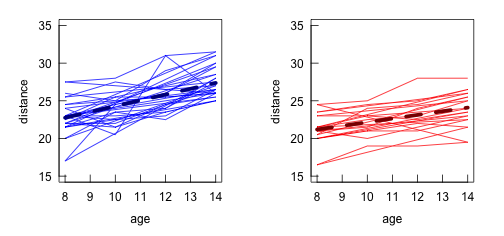
\includegraphics[width=0.9\textwidth]{lectures/day_6_praxis_and_fitting_of_mems/figures/unnamed-chunk-12-1.png}
    \tiny
    \begin{VerbatimIN}[numbers=left,numbersep=6pt]
newdata.gls <- data.frame(age = rep(seq(8,14,0.1), 2), 
                          Sex = factor(rep(c("Male","Female"),each = 61)))
predictions.gls <- predict(mod.gls, newdata.gls)
par(mfrow = c(1,2), las = 1, pty = "s", tcl = 0.5, mgp = c(2.0,0.5,0))

plot(distance ~ age, Orthodont[1:64,], xlim=c(8,14), ylim=c(15,35), type="l", col="blue")
lines(seq(8,14,0.1), as.vector(predictions.gls)[1:61], lwd=5, lty=2, col="darkblue")
plot(distance ~ age, Orthodont[65:108,], xlim=c(8,14), ylim=c(15,35), type="l", col="red")
lines(seq(8,14,0.1), as.vector(predictions.gls)[62:122], lwd=5, lty=2, col="darkred")                
    \end{VerbatimIN}[numbers=left,numbersep=6pt]
\end{frame}

\begin{frame}[fragile]
    \frametitle{}
    \huge\color{purple}\textbf{Let's try a Mixed Effect Model!}
\end{frame}

\begin{frame}
    \frametitle{The recipe to a good model}
    \begin{itemize}
        \item[] \textbf{True for all models:}
        \item define the deterministic part of the model, i.e. find the fixed effects incl. their interactions and potential quadratic / cubic etc. terms.
        \item choose a distribution for the errors
        \item[] 
        \item[] \textbf{Additionally for Mixed Effect Models:}
        \item spot the grouping in the data
        \item how many random effects are there in the data?
        \item if two or more, are they nested or crossed?
        \item can you specify random slopes / random contrasts for one or all of the random effects?
    \end{itemize}
\end{frame}

\begin{frame}
    \frametitle{Can you spot the ingredients?}
    \begin{columns}
        \begin{column}{0.5\textwidth}
            \begin{itemize}
                \item spot the grouping in the data
                \item how many random effects are there in the data?
                \item if two or more, are they nested or crossed?
                \item can you specify random slopes / random contrasts for one or all of the random effects?
            \end{itemize}
        \end{column}
        \begin{column}{0.5\textwidth}
            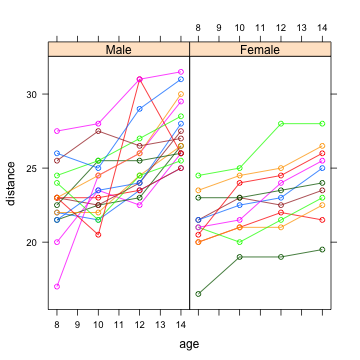
\includegraphics[width=\textwidth]{lectures/day_6_praxis_and_fitting_of_mems/figures/unnamed-chunk-14-1.png}
        \end{column}
    \end{columns}
\end{frame}

\begin{frame}[fragile]
    \frametitle{Fitting a Linear Mixed Effects Model}
    In R, we fit linear mixed effect regression models using the \textit{lme4} package:
    \scriptsize
    \begin{VerbatimIN}[numbers=left,numbersep=6pt]
mod.lmer.1 <- 
lmer(distance ~ I(age-8) * Sex + (I(age-8)|Subject))        
    \end{VerbatimIN}[numbers=left,numbersep=6pt]
    \normalsize
    Notice the subtraction of the minimum age of 8 years from the age-variable. The fixed effect Sex is now interpreted as the difference in size among boys and girls NOT at age = 0 years, but at age = 8 years, which is more meaningful for this data .
    The same interpretation of course holds true for a random slope as well.
\end{frame}

\begin{frame}[fragile]
    \frametitle{Extracting Variance Components}
    From the G-side matrix: The parameters for the variances of the random intercept, random slope, their correlations.
    From the R-side matrix: The residual variance. They are all expressed here as standard deviation, square that to get the variances.
    \scriptsize
    \begin{VerbatimIN}[numbers=left,numbersep=6pt]
VarCorr(mod.lmer.1)        
    \end{VerbatimIN}[numbers=left,numbersep=6pt]
    \begin{VerbatimOUT}[numbers=left,numbersep=6pt]
 Groups   Name        Std.Dev. Corr  
 Subject  (Intercept) 1.79832        
          I(age - 8)  0.18034  -0.091
 Residual             1.31004               
    \end{VerbatimOUT}[numbers=left,numbersep=6pt]
    \begin{VerbatimIN}[numbers=left,numbersep=6pt]
1.7983231^2    
    \end{VerbatimIN}[numbers=left,numbersep=6pt]
    \begin{VerbatimOUT}[numbers=left,numbersep=6pt]
[1]  3.233966        
    \end{VerbatimOUT}[numbers=left,numbersep=6pt]
    \normalsize
    We square the SD for the random intercept, which is the variance of the random intercept at age = 8, due to the centering.
\end{frame}

\begin{frame}[fragile]
    \frametitle{Extracting Variance Components}
    \textbf{The Variance-Covariance Matrix of Parameters:}
    \vspace{0.3cm}

    \scriptsize
    \begin{VerbatimIN}[numbers=left,numbersep=6pt]
round(vcov(mod.lmer.1), 2)        
    \end{VerbatimIN}[numbers=left,numbersep=6pt]
    \tiny
    \begin{VerbatimOUT}[numbers=left,numbersep=6pt]
4 x 4 Matrix of class "dpoMatrix"
                     (Intercept) I(age - 8) SexFemale I(age - 8):SexFemale
(Intercept)                 0.28      -0.02     -0.28                 0.02
I(age - 8)                 -0.02       0.01      0.02                -0.01
SexFemale                  -0.28       0.02      0.68                -0.04
I(age - 8):SexFemale        0.02      -0.01     -0.04                 0.02     
    \end{VerbatimOUT}[numbers=left,numbersep=6pt]
\end{frame}

\begin{frame}[fragile]
    \frametitle{Combined Variance-Covariance Matrix of Residuals}
    \scriptsize
    \begin{VerbatimIN}[numbers=left,numbersep=6pt]
# get components
var.d <- crossprod(getME(mod.lmer.1,"Lambdat")) # based on BLUPs
Zt <- getME(mod.lmer.1,"Zt") # transposed model matrix
vres <- sigma(mod.lmer.1)^2 # residual variance
# combine them
var.b <- (t(Zt) %*% var.d %*% Zt)
sI <- vres * Diagonal(nrow(Orthodont))
var.y <- var.b + sI
image(var.y)
    \end{VerbatimIN}[numbers=left,numbersep=6pt]

    \begin{center}
        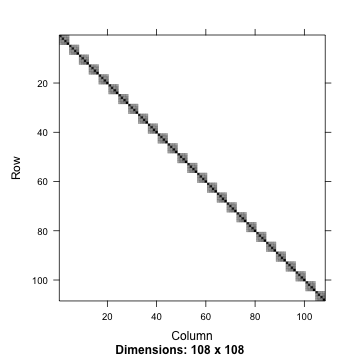
\includegraphics[width=0.4\textwidth]{lectures/day_6_praxis_and_fitting_of_mems/figures/unnamed-chunk-19-1.png}
    \end{center}
\end{frame}

\begin{frame}[fragile]
    \frametitle{Now let's have a look at the full model summary}
    \scriptsize
    \begin{VerbatimIN}[numbers=left,numbersep=6pt]
summary(mod.lmer.1)        
    \end{VerbatimIN}[numbers=left,numbersep=6pt]
    \tiny
    \begin{VerbatimOUT}[numbers=left,numbersep=6pt]
Linear mixed model fit by REML ['lmerMod']
Formula: distance ~ I(age - 8) * Sex + (I(age - 8) | Subject)

REML criterion at convergence: 432.6
Scaled residuals: 
    Min      1Q  Median      3Q     Max 
-3.1681 -0.3859  0.0071  0.4452  3.8495 
Random effects:
 Groups   Name        Variance Std.Dev. Corr 
 Subject  (Intercept) 3.23394  1.7983        
          I(age - 8)  0.03252  0.1803   -0.09
 Residual             1.71621  1.3100        
Number of obs: 108, groups:  Subject, 27
Fixed effects:
                     Estimate Std. Error t value
(Intercept)           22.6156     0.5265  42.954
I(age - 8)             0.7844     0.0860   9.121
SexFemale             -1.4065     0.8249  -1.705
I(age - 8):SexFemale  -0.3048     0.1347  -2.262
Correlation of Fixed Effects:
            (Intr) I(g-8) SexFml
I(age - 8)  -0.396              
SexFemale   -0.638  0.253       
I(g-8):SxFm  0.253 -0.638 -0.396        
    \end{VerbatimOUT}[numbers=left,numbersep=6pt]
\end{frame}

\begin{frame}
    \frametitle{The Random Effects Structure}
    \large\textbf{Keep it maximal:}
    \vspace{0.5cm}
    
    \normalsize{"We show that LMMs generalize best when they include the maximal random effects structure justified by the design. Random-intercepts-only LMMs used on within-subjects data from populations where subjects vary in their sensitivity to experimental manipulations always generalize worse. Maximal LMMs should be the 'gold standard' for confirmatory hypothesis testing."}
    \vspace{1cm}
    \small\href{https://europepmc.org/backend/ptpmcrender.fcgi?accid=PMC3881361&blobtype=pdf}{Barr, D. J.; Levy, R.; Scheepers, C. \& Tily, H. J. (2013) Random effects structure for confirmatory hypothesis testing: Keep it maximal. Journal of Memory and Language, 68, 255-278.} 
\end{frame}

\begin{frame}[fragile]
    \frametitle{Random effect structures}
    \textbf{Random Intercept - Random Slope}
    \scriptsize
    \begin{VerbatimIN}[numbers=left,numbersep=6pt]
mod.lmer.1 <- 
lmer(distance ~ I(age-8) * Sex + (I(age-8) | Subject))
# in line with the KEEP IT MAXIMAL principle

VarCorr(mod.lmer.1)        
    \end{VerbatimIN}[numbers=left,numbersep=6pt]
    \begin{VerbatimOUT}[numbers=left,numbersep=6pt]
 Groups   Name        Std.Dev. Corr  
 Subject  (Intercept) 1.79832        
          I(age - 8)  0.18034  -0.091
 Residual             1.31004          
    \end{VerbatimOUT}[numbers=left,numbersep=6pt]
\end{frame}

\begin{frame}[fragile]
    \frametitle{Random Intercept - Random Slope...}
    \textbf{... without correlation between random effects parameters}
    \scriptsize
    \begin{VerbatimIN}[numbers=left,numbersep=6pt]
mod.lmer.2 <- 
lmer(distance ~ I(age-8) * Sex + (I(age-8) || Subject))
# no correlation, not the double vertical bar

VarCorr(mod.lmer.2)        
    \end{VerbatimIN}[numbers=left,numbersep=6pt]
    \begin{VerbatimOUT}[numbers=left,numbersep=6pt]
 Groups    Name        Std.Dev.
 Subject   (Intercept) 1.76496 
 Subject.1 I(age - 8)  0.16953 
 Residual              1.31747         
    \end{VerbatimOUT}[numbers=left,numbersep=6pt]
\end{frame}

\begin{frame}[fragile]
    \frametitle{Random Intercept Only}
    \scriptsize
    \begin{VerbatimIN}[numbers=left,numbersep=6pt]
mod.lmer.3 <- 
lmer(distance ~ I(age-8) * Sex + (1 | Subject))
# violates the KEEP IT MAXIMAL principle

VarCorr(mod.lmer.3)
    \end{VerbatimIN}[numbers=left,numbersep=6pt]
    \begin{VerbatimOUT}[numbers=left,numbersep=6pt]
 Groups   Name        Std.Dev.
 Subject  (Intercept) 1.8162  
 Residual             1.3864  
    \end{VerbatimOUT}[numbers=left,numbersep=6pt]
\end{frame}

\begin{frame}[fragile]
    \frametitle{More on Random Effects Structures}
    \Large
    \color{blue}\href{https://stats.stackexchange.com/questions/13166/rs-lmer-cheat-sheet?lq=1}{R's lmer cheat sheet}
    \vspace{0.5cm}
    
    \color{blue}\href{http://bbolker.github.io/mixedmodels-misc/glmmFAQ.html#model-specification}{GLMM FAQ: Model specification}
\end{frame}

\begin{frame}
    \frametitle{}
    \centering
    \huge\color{purple}\textbf{Break!}
\end{frame}

\begin{frame}[fragile]
    \frametitle{Predictions with LMM}
    \textbf{We need to give the new design matrix a vector for the levels of the Random Effects}
    \scriptsize
    \begin{VerbatimIN}[numbers=left,numbersep=6pt]
newdata.lmer <- data.frame(
 age = rep(seq(8, 14, 0.1), 27), # 61 new age values
 Sex = c(rep("Male", 16 * 61), rep("Female", 11 * 61)),
 Subject = rep(levels(Orthodont$Subject), each = 61),
 # one for the identity of the 27 children measured
 distance = rep(NA, 27 * 61))        
    \end{VerbatimIN}[numbers=left,numbersep=6pt]
\end{frame}

\begin{frame}[fragile]
    \frametitle{}
    Set re.form = NA or re.form = ~ 0 for the population-average predictions, \textbf{marginalising} over the random effects levels (i.e. setting random effects to zero)
    \scriptsize
    \begin{VerbatimIN}[numbers=left,numbersep=6pt]
newdata.lmer$distance <- 
predict(mod.lmer.1, newdata.lmer, re.form = NA)
xyplot(distance ~ age | Subject, 
data = newdata.lmer, type = "l", lwd = 3)
    \end{VerbatimIN}[numbers=left,numbersep=6pt]
    \begin{center}
       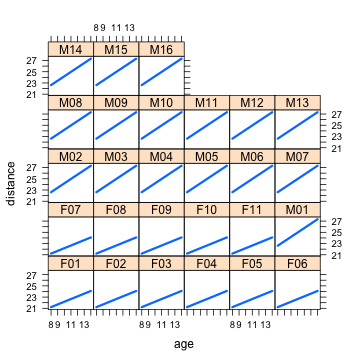
\includegraphics[width=0.5\textwidth]{lectures/day_6_praxis_and_fitting_of_mems/figures/unnamed-chunk-25-1.png} 
    \end{center}
\end{frame}

\begin{frame}[fragile]
    \frametitle{}
    In contrast to the predictions of random effects levels (i.e. the BLUPs), re.form = NULL \textbf{conditions} on all random effects, re.form = (1 $|$ Subject) on Subject only, etc.
    \scriptsize
    \begin{VerbatimIN}[numbers=left,numbersep=6pt]
newdata.lmer$distance <- 
predict(mod.lmer.1, newdata.lmer, re.form = NULL)
xyplot(distance ~ age|Subject, 
data=newdata.lmer, type="l", lwd=3)
    \end{VerbatimIN}[numbers=left,numbersep=6pt]
    \begin{center}
       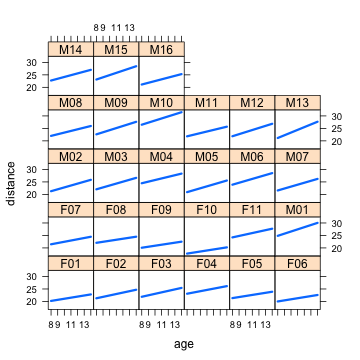
\includegraphics[width=0.5\textwidth]{lectures/day_6_praxis_and_fitting_of_mems/figures/unnamed-chunk-26-1.png} 
    \end{center}
\end{frame}

\begin{frame}
    \frametitle{}
    \textbf{Confidence intervals of population-trend WITHOUT random effects. Who remembers the steps from the second day?}
    \vspace{0.5cm}
    
    \begin{itemize}
        \item Create new design matrix $\mathit{X}$ and matrix multiply $\mathit{X}$ and $\mathit{\beta}$ to get predictions
        \item Extract the variance-covariance matrix of parameters $\mathit{V}$
        \item Compute $\mathit{XV X'}$ for variance-covariance matrix of predictions
        \item Extract diagonal to get variances and the square root to get standard errors
        \item Compute confidence interval based on normal approximation
    \end{itemize}
\end{frame}

\begin{frame}[fragile]
    \frametitle{Confidence Intervals of Population-Trend}
    \textbf{WITHOUT random effects}
    \scriptsize
    \begin{VerbatimIN}[numbers=left,numbersep=6pt]
newdata.lmer$distance <- 
predict(mod.lmer.1, newdata.lmer, re.form = NA)
# new design matrix
X <- model.matrix(terms(mod.lmer.1), newdata.lmer) 
XVX <- X \%*\% vcov(mod.lmer.1) \%*\% t(X) 
# calculate SE
se <- sqrt(diag(XVX)) 
conf <- se * 1.96 
# normal approximation to get confidence intervall

newdata.lmer <- data.frame(newdata.lmer,
    lo = newdata.lmer$distance - conf, 
    hi = newdata.lmer$distance + conf)        
    \end{VerbatimIN}[numbers=left,numbersep=6pt]
\end{frame}

\begin{frame}[fragile]
    \frametitle{Confidence Intervals for Population-Trend}
    \textbf{WITHOUT random effects}

    \begin{center}
        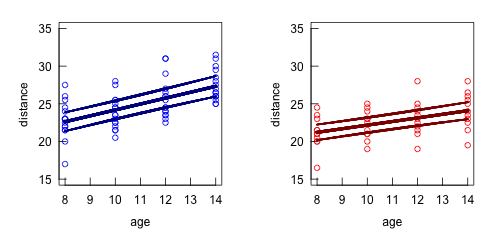
\includegraphics[width=\textwidth]{lectures/day_6_praxis_and_fitting_of_mems/figures/unnamed-chunk-28-1.png}
    \end{center}
    
    \textbf{The confidence interval here only accounts for the fixed effects uncertainty}
\end{frame}

\begin{frame}[fragile]
    \frametitle{Confidence Intervals of Population-Trend}
    \textbf{WITH random effects}
    \scriptsize
    \begin{VerbatimIN}[numbers=left,numbersep=6pt]
X <- model.matrix(terms(mod.lmer.1), newdata.lmer[,1:4]) 
# new design matrix
XVX <- X %*% vcov(mod.lmer.1) %*% t(X) 

# now add effects from Random Effects parameters 
# (variances) but NOT uncertainty of RE parameters 
#(variance of variances)
vari <- diag(XVX) + VarCorr(mod.lmer.1)$Subject[1]  
# calculate SE
se <- sqrt(vari)           
conf <- se * 1.96 
# normal approximation to get confidence intervall

newdata.lmer$lo <- newdata.lmer$distance - conf
newdata.lmer$hi <- newdata.lmer$distance + conf        
    \end{VerbatimIN}[numbers=left,numbersep=6pt]
\end{frame}

\begin{frame}[fragile]
    \frametitle{Confidence Intervals for Population-Trend}
    \textbf{WITH random effects}

    \begin{center}
        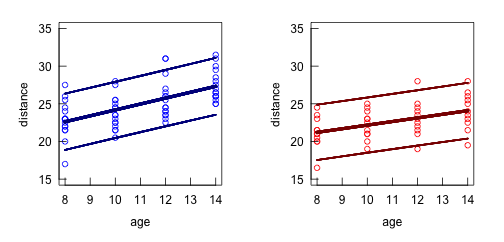
\includegraphics[width=\textwidth]{lectures/day_6_praxis_and_fitting_of_mems/figures/unnamed-chunk-30-1.png}
    \end{center}
\end{frame}

\begin{frame}[fragile]
    \frametitle{}
    \textbf{For predictions of Random Effects levels, set re.form = random effects structure or re.form = NULL}
    \scriptsize
    \begin{VerbatimIN}[numbers=left,numbersep=6pt]
newdata.lmer$distance <- 
predict(mod.lmer.1, newdata.lmer, re.form =  NULL)

# newdata.lmer$distance <- 
# predict(mod.lmer.1, newdata.lmer, 
# re.form =  ~ (age|Subject))        
    \end{VerbatimIN}[numbers=left,numbersep=6pt]
\end{frame}

\begin{frame}[fragile]
    \frametitle{}
    \begin{center}
        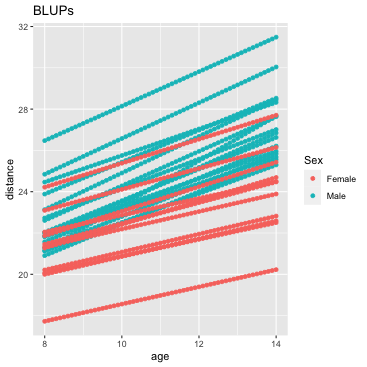
\includegraphics[width=0.7\textwidth]{lectures/day_6_praxis_and_fitting_of_mems/figures/unnamed-chunk-32-1.png}
    \end{center}
\end{frame}

\begin{frame}[fragile]
    \frametitle{}
    \textbf{Confidence intervalls of point estimates of Random Effects levels (BLUPs)}
    \scriptsize
    \begin{VerbatimIN}[numbers=left,numbersep=6pt]
cV <- ranef(mod.lmer.1, condVar = TRUE) 
# Assumed identical for each BLUP. This gives the confidence 
#interval for the intercepts and slopes for each child.  
library(lattice)
dotplot(cV)         
    \end{VerbatimIN}[numbers=left,numbersep=6pt]
    \begin{center}
        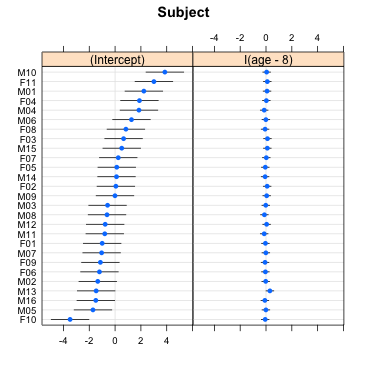
\includegraphics[width=0.5\textwidth]{lectures/day_6_praxis_and_fitting_of_mems/figures/unnamed-chunk-33-1.png}
    \end{center}
\end{frame}

\begin{frame}[fragile]
    \frametitle{For more code see:}
    \Large
    \color{blue}\href{http://bbolker.github.io/mixedmodels-misc/glmmFAQ.html}{FAQ list by B Bolker, co-developer of lme4 package}
\end{frame}

\begin{frame}[fragile]
    \frametitle{Syntax for library(nlme)}
    \textbf{There is a second R-package we use:}
    \scriptsize
    \begin{VerbatimIN}[numbers=left,numbersep=6pt]
mod.lme.1 <- 
lme(distance~I(age-8) * Sex, random = ~ I(age-8)|Subject)
# random slope and intercept

mod.lme.2 <- 
lme(distance~I(age-8) * Sex, random = ~ 1|Subject)
# random intercept only        
    \end{VerbatimIN}[numbers=left,numbersep=6pt]

\end{frame}

\begin{frame}[fragile]
    \frametitle{nlme vs lme4}
    \textbf{Differences:}
    \begin{itemize}
        \item REML is differently turned on and off
        \item Marginalizing over Random Effects levels in predict function
        \item nlme() allows for correlations of data points
        \item nlme easy for Heterogeneous Variance models (not covered!)
        \item lme4() can fit GLMMs
        \item lme4() easy for crossed Random Effects
        \item Intervals() in nlme() gives approximate confidence intervals for parameters
        \item Confint() in lme4() gives Likelihood CI profiles or bootstrapped CI
        \item nlme() gives p-values which are likely \textbf{wrong}
        \item lme4() does not give p-values
    \end{itemize}
\end{frame}

\begin{frame}
    \frametitle{Recap of Week 6}
    \textbf{Today's content was using library(nlme) and library(lme4) to fit Linear Mixed Effects Models}
    \vspace{0.5cm}
    
    \begin{itemize}
        \item \textbf{Syntax} differences among two packages
        \item Using \textbf{VarCorr} to extract Random Effects parameters
        \item The various \textbf{Random Effects structures}
        \item Predictions of population avarage with and without \textbf{RE uncertainty}
        \item Predictions of \textbf{BLUPs}
        \item Extracting the residual covariance matrix
    \end{itemize}
    \vspace{0.5cm}
    
    Today after lecture: Exercises on fitting mixed effects models with nlme and lmer in R.
\end{frame}

\end{document}